\documentclass[a4paper]{article}
\usepackage[utf8x]{inputenc}
\usepackage[brazil]{babel}
\usepackage[T1]{fontenc}
\usepackage{graphicx}

\begin{document}

\begin{titlepage}
 \vfill
  \begin{center}
   {\large \textbf{CENTRO UNIVERSITÁRIO SENAC}} \\
   {\large \textbf{BACHARELADO EM CIÊNCIA DA COMPUTAÇÃO}} \\[4cm]
   
   {\large \textbf{GABRIEL VIEIRA FIGUEIREDO TOMAZ}}\\
   {\large \textbf{TALES CARLOS DE PÁDUA}}\\
   {\large \textbf{VINICIUS DE CARVALHO}}\\[4cm]


   {\Large Mini Games com Visão Computacional}\\[4cm]

\vspace{2cm}
\large \textbf{SÃO PAULO}

\large \textbf{MAIO DE 2014}
\end{center}
\end{titlepage}

\break

\begin{titlepage}
 \vfill
  \begin{center}
   {\large \textbf{CENTRO UNIVERSITÁRIO SENAC}} \\
   {\large \textbf{BACHARELADO EM CIÊNCIA DA COMPUTAÇÃO}} \\[4cm]

   {\large \textbf{Gabriel Vieira Figueiredo Tomaz, Tales Carlos de Pádua, Vinicius de Carvalho.}}\\ [1cm]
  
   {\large \textbf{viera\_frifri@hotmail.com, talescpadua@gmail.com, carvalho.v@outlook.com.}}\\ [3cm]
   
 
   {\Large Mini Games com Visão Computacional}\\[2cm]

   \hspace{.45\textwidth} 
   \begin{minipage}{.5\textwidth}
   \large "Pequenos jogos eletrônicos utilizando conhecimentos de Visão Computacional apresentados para a conclusão da disciplina Projeto Interativo III, do bacharelado em Ciência da Computação, Centro Universitário Senac."\\[0.5cm]
			Sob orientação do Prof.º: Marcelo Hashimoto
  \end{minipage}
  \vfill

\vspace{1cm}
\large \textbf{SÃO PAULO}

\large \textbf{MAIO DE 2014}
\end{center}
\end{titlepage}




\section{Resumo}


Conforme proposto na disciplina de Projeto Interativo III, a partir do estudo de algoritmos relacionados à visão computacional foram desenvolvidos pequenos jogos eletrônicos (mini games) em linguagem C usando a interface gráfica provida pela biblioteca Allegro 5 e uma interface de acesso à câmeras de vídeo provida pela biblioteca OpenCV, de modo que a visão computacional oferecesse não apenas uma opção de controle para o jogador, mas sim um diferencial na experiência e imersão do usuário ao vivenciar os mini games.\\

Palavras-chave: jogos eletrônicos, visão computacional, Allegro 5.\\	



\section{Abstract}


As proposed by the Interactive Project III discipline, from the study of algorithms related to computer vision were originated little eletronic games (mini games) in C language utilizing a graphical interface provided by Allegro 5 library and a web cam access interface provided by OpenCV library, in order to make computer vision offer not only another controller option for the player, but a different experience and imersion for the user while playing the mini games.\\

Keywords: eletronic games, computer vision, Allegro 5.\\



\section {Introdução}


A visão computacional é uma ciência e tecnologia voltada a lidar com a forma como as máquinas enxergam o mundo ao seu redor. As informações captadas por meio de sensores (como scanners, câmeras de vídeo, etc.) podem ser modeladas de diversas formas a fim de suprir necessidades que permeiam desde ramos diretamente ligados à tecnologia de informação (como robótica e áreas de automação tecnológica) até os que se utilizam da tecnologia para dadas outras necessidades, como ciências ambientais, medicina e outros.\\

Com o objetivo de dar um passo inicial para dentro da visão computacional, este trabalho visa utilizar técnicas e algoritmos da mesma aliada à captação de imagens por câmera de vídeo para a produção de jogos simples, mas que mantenham a jogabilidade focada no poder da visão computacional, de modo que a experiência do jogador, ao invés de ser restringida pela interface proposta, se torne um diferencial por conta deste quesito.



\section{Desenvolvimento}



\textbf{\large Ponto de Partida}


Visto que este trabalho foi o primeiro contato formal com a visão computacional por parte do grupo, a estatégia adotada desenvolver os mini games foi uma via de mão-dupla passando por um \textit{brainstorm} de jogos existentes até quais algoritmos poderiam modelar uma interface de controle aceitável para os mesmos e fazendo o caminho de volta, onde eram estudados algoritmos existentes e se imaginava o que era possível, em termos de jogos, produzir a partir deles.

A partir desta metodologia aliada à orientação e pesquisa, surgiram as tecnicas e algoritmos a seguir e a consequente combinação dos mesmos para elaboração dos jogos. 

No início do trabalho foi introduzido uma biblioteca, baseada em OpenCV, que faz a interface de acesso à câmera de maneira bem restrita, possibilitando apenas que houvesse contato com os quadros capturados da câmera fornecidos por uma matriz tridimensional onde a primeira dimensão é a altura (em pixels) da imagem, a segunda representa a largura (também em pixels) e a terceira são os componentes vermelho (red), verde (green) e azul (blue), respectivamente, do espaço de cores RGB. Todos os valores da matriz representam um número entre 0 e 255 do padrão RGB.

\begin{flushleft}
\textbf{\large Jogo Genius}
\end{flushleft}
Esse jogo consiste em um remake do classico jogo genius com a jogabilidade alterada para ser possivel jogar com imagens capturadas pela web cam.

A principal ideia do jogo se baseou no reconhecimento básico da cor vermelha, onde se era verificado se o componente R do pixel era maior que a soma dos outros dois G e B, conseguindo detectar com sucesso a cor desejada. Apesar de funcionar relativamente bem para detecção de vermelho, outras cores apresentavam uma resistência maior ao método devido a pequenas instabilidades e mudanças de luz. Sendo necessário buscar algum outro metodo que nos pudesse fornecer uma melhor precisão nesse reconhecimento . Dentre alguns pesquisados , a solução adotada foi a conversão do espaço de cor RGB para o HSV pois com ele, definir um range e uma intensidade para a detecção de uma cor especifica fica muito mais preciso e intuitivo , devido suas caracteristicas unicas.


\vspace{5.00mm}
\centering

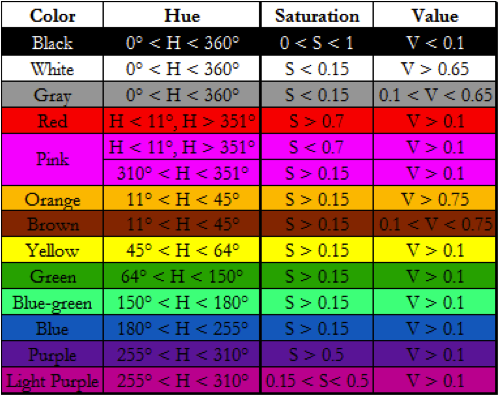
\includegraphics[scale=0.8]{scale.png}
\centering
\\
\textbf{\normalsize Range das cores em HSV}

\begin{flushleft}
\textbf{\large Espaço de cor HSV}
\end{flushleft}
\raggedright
 O sistema de cores HSV formadas pelas componentes Hue (tonalidade), Saturation (Saturação) e Value (Valor). Esse sistema também é conhecido como HSB (Hue, Saturation e Brightness - Tonalidade, Saturação e Brilho, respectivamente). A primeira componente H define a cor propriamente dita , podendo varias de 0 a 360 graus , a ssegunda componente S defini a pureza ou intesidade da cor 
contida na componente H e por ultimo a componente V defini o brilho da componente H.

\vspace{5.00mm}
\centering

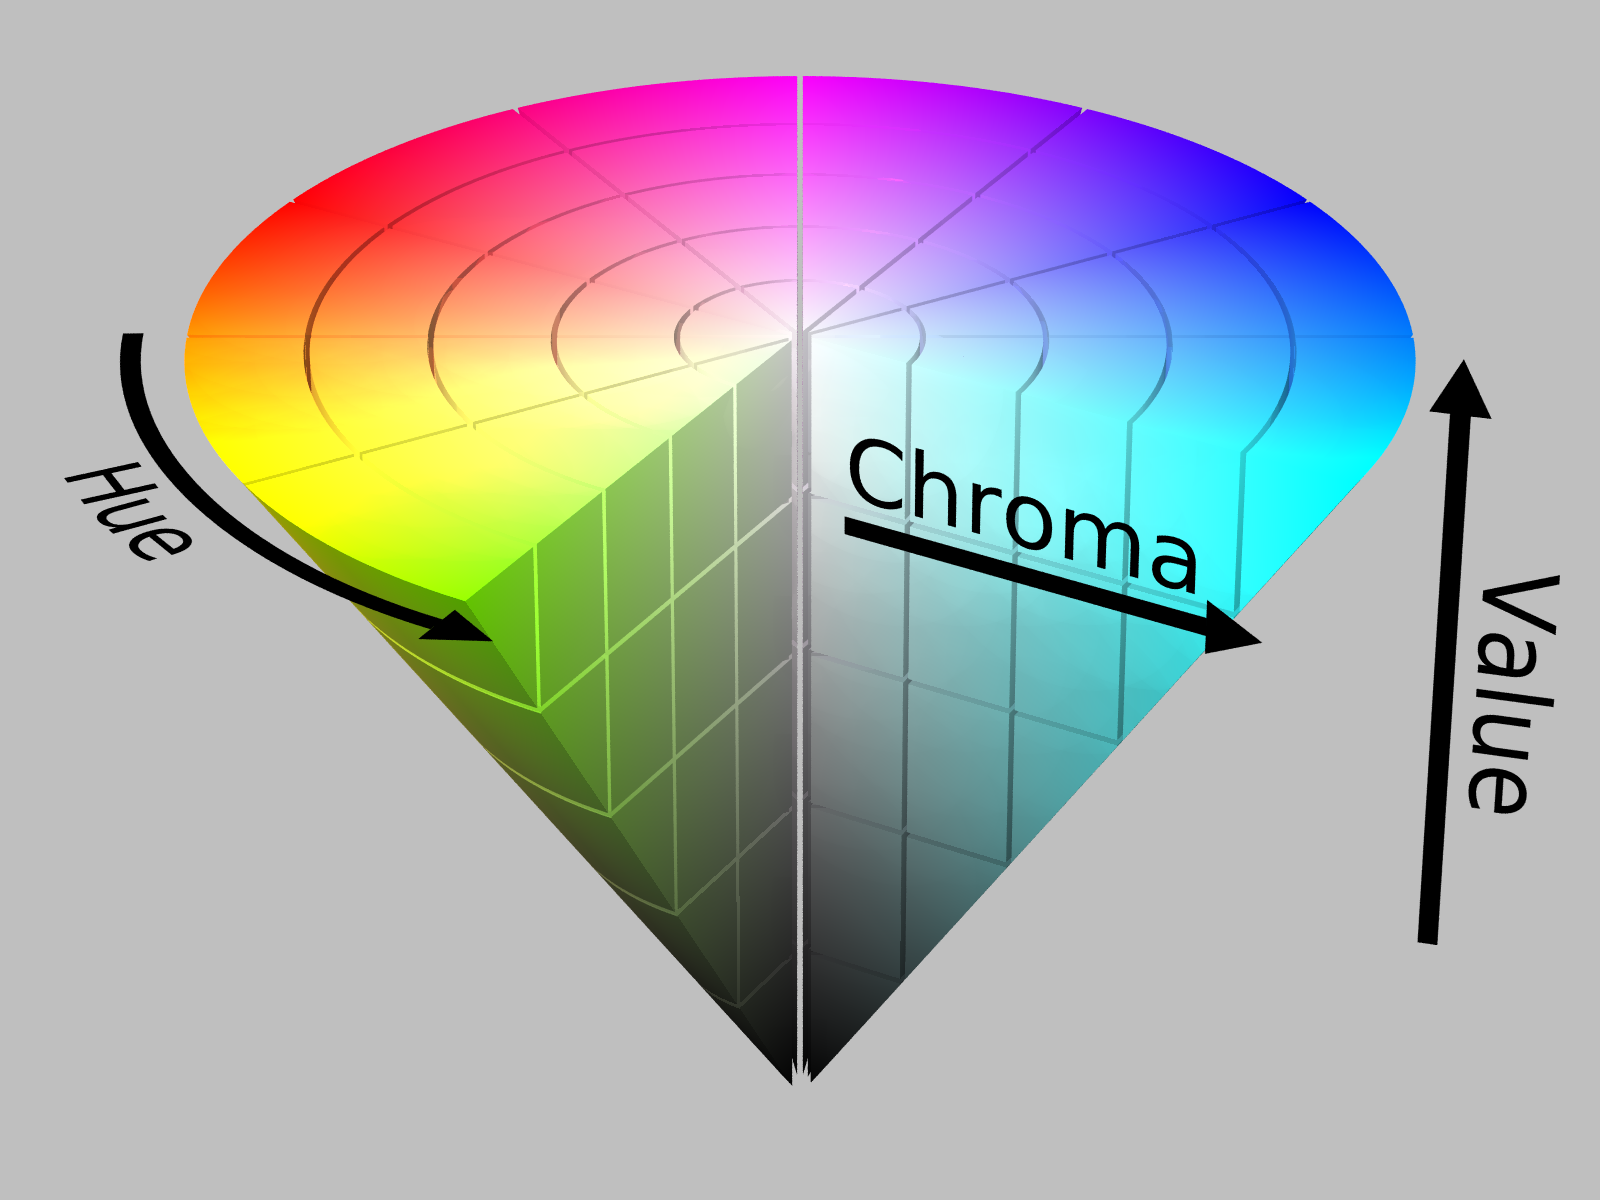
\includegraphics[scale=0.08]{hsv.png}
\\
\centering
\textbf{\normalsize Espaço de cor HSV}
\vspace{5.00mm}

Como resultado da convesão para esse espaço de cor podemos ver um exemplo da detecção de azul :

\vspace{5.00mm}
\centering
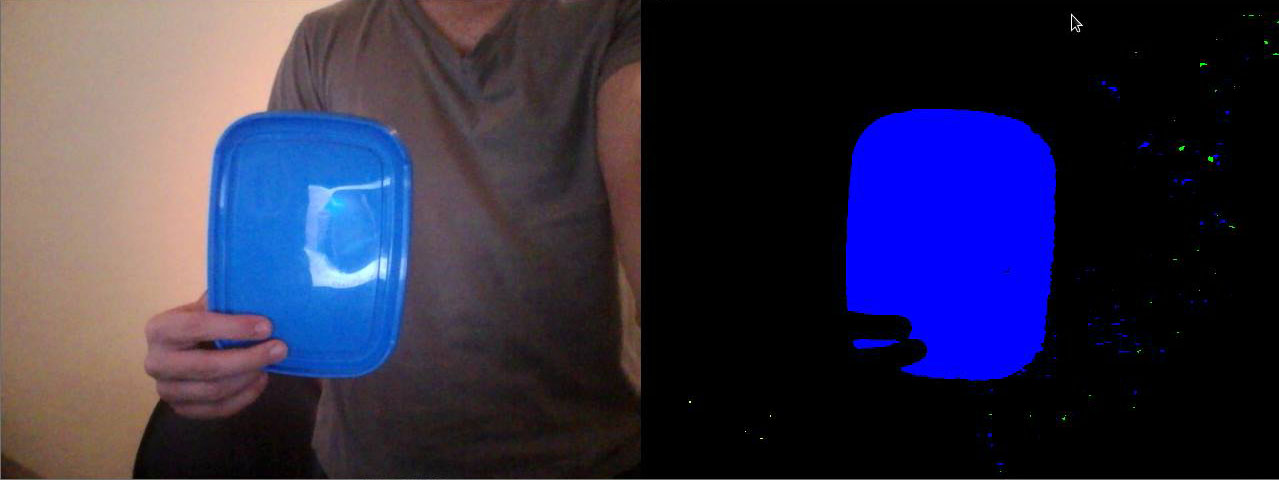
\includegraphics[scale=0.3]{img2.jpg}

\vspace{5.00mm}


\begin{flushleft}
\textbf{\large Jogo: Sorvete Hoje?}
\end{flushleft}
\raggedright
%%explicar ideia do jogo antes

A ideia deste jogo surgiu a partir do estudo de certos algoritmos que aliados permitem uma detecção de borda, que foi a base para a detecção de face. A detecção desta borda é feita por meio de um Filtro de Sobel, que será explicado mais adiante. Aliado ao filtro, para que houvessem bordas mais consistentes, foi utilizado um algoritmo de binarização de imagem. A técnica utilizada é conhecida como algoritmo de Otsu.

Apenas o filtro, porém, não era suficiente para atingir os objetivos, visto que a manipulação de quadros da câmera pode ser um processo bastante custoso, o que gera uma experiência ruim para o usuário. Visando um modo de se otimizar este processo, antes de se aplicar o algoritmo do filtro foi utilizada uma conversão da imagem para escala de cinza.

Por fim, para evitar impecilhos com a imagem de fundo da câmera, também foi agregado um algoritmo de remoção de fundo simples utilizando a fórmula matemática da Distância Euclidiana nos pixels dos quadros.

\begin{flushleft}
\textbf{\large Distância Euclidiana}
\end{flushleft}
\%\% TODO: distância euclidiana


\begin{flushleft}
\textbf{\large Escala de Cinza}
\end{flushleft}
\%\% TODO: grey scale

\begin{flushleft}
\textbf{\large Binarização}
\end{flushleft}
\%\% TODO: binarização

\begin{flushleft}
\textbf{\large Filtro Sobel}
\end{flushleft}
\%\% TODO: sobel operator para detecção de bordas

\begin{flushleft}
\textbf{\large Filtro Gaussiano}
\end{flushleft}
\%\% TODO: distância euclidiana

%\begin{figure}[!htb]
%\centering
%\includegraphics{tela_do_jogo.png}
%\caption{Figura 1 ? Tela do jogo com as cartas para a implementação dos algoritmos (Fonte: Jogo, Código de Honra criado pelo grupo ? Retirada 18/11/2013)}
%\label{Rotulo}
%\end{figure}

%\begin{figure}[!htb]
%\centering
%\includegraphics{git.png}
%\caption{Figura 2 ? Repositório do jogo criado para auxiliar o compartilhamento de dados via Web (Fonte: Github - https://github.com/tgl-dogg/BCC_PI2_CDH ? Retirada 20/11/2013)}
%\label{Rotulo}
%\end{figure}



\section{ Resultados}

Os resultados obtidos com o desenvolvimente desse trabalho nos proporcionaram um algoritmo rustico de detecção de padroes da face e outro efeciente na detecção de cores , mostrando que com a combinação de alguns algoritmos simples de uma maneira inteligente é possivel chegar em grandes resultados. Resultados esses que podemos ver nos jogos criados que conseguem exercer seus objetivos com eficiencia e precisão.

Ao longo desse trabalho, foi possível obtermos uma visão de alguns dos problemas no campo da visão computacional e da geometria computacional, casos em que demandavam uma maior atenção no desenvolvimento de seus algorítmos, além de cuidado na performance em que algoritmos destes ramos demandam.


\section{Conclusão}


Existem diversas formas de se trabalhar com visão computacional e mesmo limitando o escopo de trabalho para produzir apenas jogos, foi possível estudar e aplicar conceitos bastante diferentes entre si, como mudanças de espaço de cor e métodos de tratamento de imagem para reconhecimento de padrões. Apesar de não serem as técnicas mais sofisticadas, todos os algoritmos descritos atenderam as necessidades de cada jogo e assim foi possível criar uma experiência de usuário realmente inovadora tanto para um jogo clássico, como o \textit{Genius}, quanto para um jogo independente, como o caso do \textit{Sorvete Hoje?}. 


\section{ Referências Bibliográficas}


\%\% TODO formatar referências em ABNT \\
- Livros do nosso Google Drive sobre Visão Computacional \\
- Livro de Álgebra Linear da aula da Dani com a distância euclidiana \\
- Tutoriais do OpenCV \\

%% um pouco de introdução à computer vision eu tirei daqui:
%% http://en.wikipedia.org/wiki/Computer_vision

\break

\end{document}